\section{Correlation of Performance Metrics}
\label{sec:appendix/correlation}

We examined the video sequences with each performance metric, and some metrics are defined in terms of other metrics according to the definitions listed in Chapter \ref{sec:background/section_d}. We did not explicitly describe which metrics correlate or relate to other metrics but included the following figure, the potentially useful information to reveal the correlation between different performance metrics. Figure \ref{fig:correlation} shows the heatmap of correlation between different metrics, varying the QP values. The result is based on 12 video samples on the "person" object class, fixing at MSR = 16.

The potential useful insights are, for example, MOTA is defined in terms of FN, FP, IDs, and GT. From the correlation heatmap, excluding the constant GT, FN correlates the most compared to FP and IDs. This explains why the increase of FN is significantly larger than the change of FP and IDs so that MOTA decreases. FP still correlates significantly with MOTA but IDs correlates little. The p-value of correlation between MOTA and IDs is 0.44, therefore IDs does not significantly correlate with MOTA. For IDs, FM is correlated the most. This is logical since the ID switch happens when the object gets undetected and re-detected, while FM occurs when the object state changes from detected to undetected, losing on the track. IDP is also negatively correlated significantly.
\begin{figure}[!htbp]
  \centering
  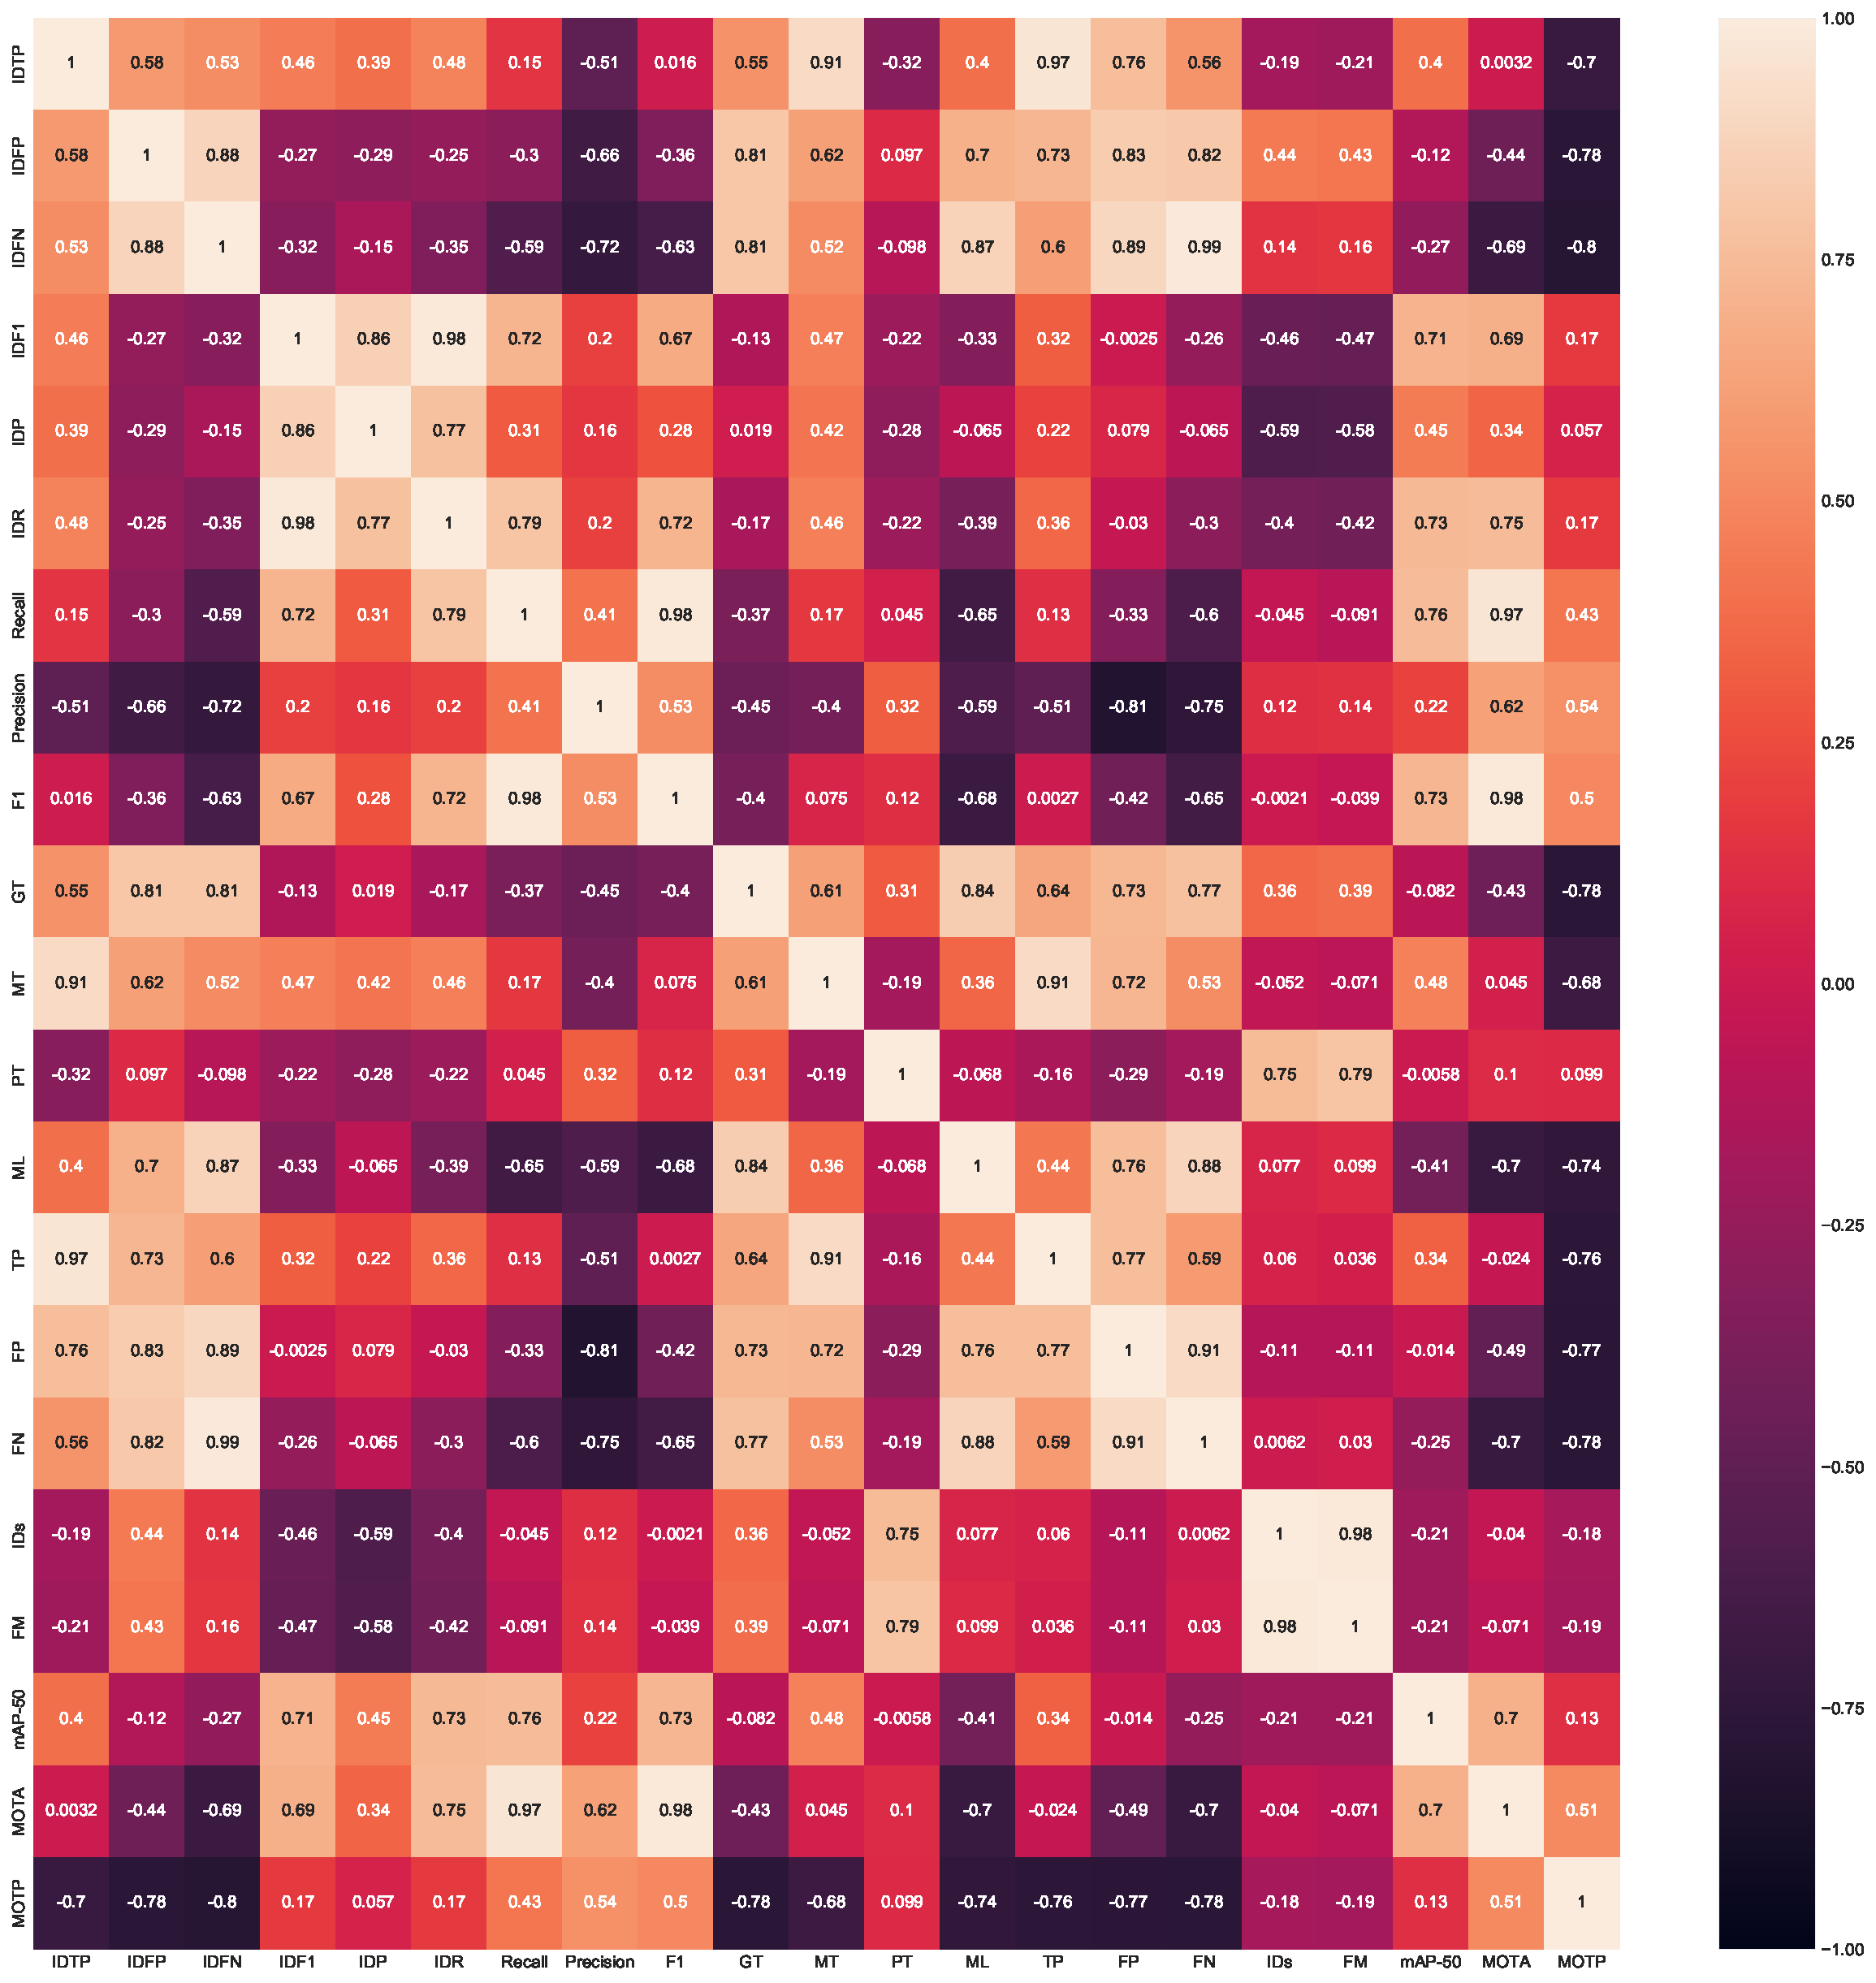
\includegraphics[width=1.0\linewidth]{img/correlation.pdf}
  \caption[Pearson correlation heatmap of performance metrics for "all" object classes]
  {
  Pearson correlation heatmap of performance metrics for "all" object classes.
  }
  \label{fig:correlation}
\end{figure}